%Unless you substantially alter a figure, you are not allowed to use figures from a published document, including journal articles, without copyright permission from the publisher.  This is usually easily secured, without cost to you.  Go to the journal article or book on the publisher's website, and find the Copyrights/Permissions link.  Just fill out the form or follow instructions, and you will be emailed documentation of permission to use the figure in your thesis.  For more information on using copyrighted figures in your thesis, see 

%\href{http://guides.lib.umich.edu/dissertationcopyright/otherscontent}{http://guides.lib.umich.edu/dissertationcopyright/otherscontent}.

%You can include the copyright permissions in an appendix as figures or include a pdf using this command \verb!\includepdf[scale=0.9]{rsna.pdf}!. If you do this, you could reference the appendix in each figure caption with ``(See Appendix B for documentation of permission to republish from [cite source].)" Alternatively, you can save your permission documents into a separate document and include them as a separate upload to the \gls{cdr}.  Make sure you note in your thesis that you are using the figure with permission.  Please talk to Richard Jizba at the Creighton Library for advice.  


% ============================================================
% APPENDIX G -- Copyright Permissions
% ============================================================

This appendix contains the copyright license agreements obtained for figures reproduced in this thesis. Two figures were reproduced from previously published works and required formal permission. Figures~\ref{fig:tvleadFixation} and Figure \ref{fig:leadDesign} were reproduced from Clinical Cardiac Pacing, Defibrillation, and Resynchronization Therapy (Haqqani et al., 2011, Elsevier), and Figure~\ref{fig:astm_diagram} is reproduced from ASTM F2052-21 (ASTM International). The full license terms for each are included below as issued by the respective rights holders. 

All figures not listed below are original to this work. This includes graphs and plots generated in Python, photographs taken by the author or members of the research team at \gls{bergan}, and custom diagrams produced in Inkscape. No external permission is required to reproduce these figures for academic or educational purposes, provided proper citation of this thesis is given. Questions regarding copyright ownership of original figures produced under institutional supervision should be directed to the Creighton University Graduate School.


\invisiblesection{Appendix F1: Copyright License – Figure \ref{fig:leadFixation}}
\label{app:B1}

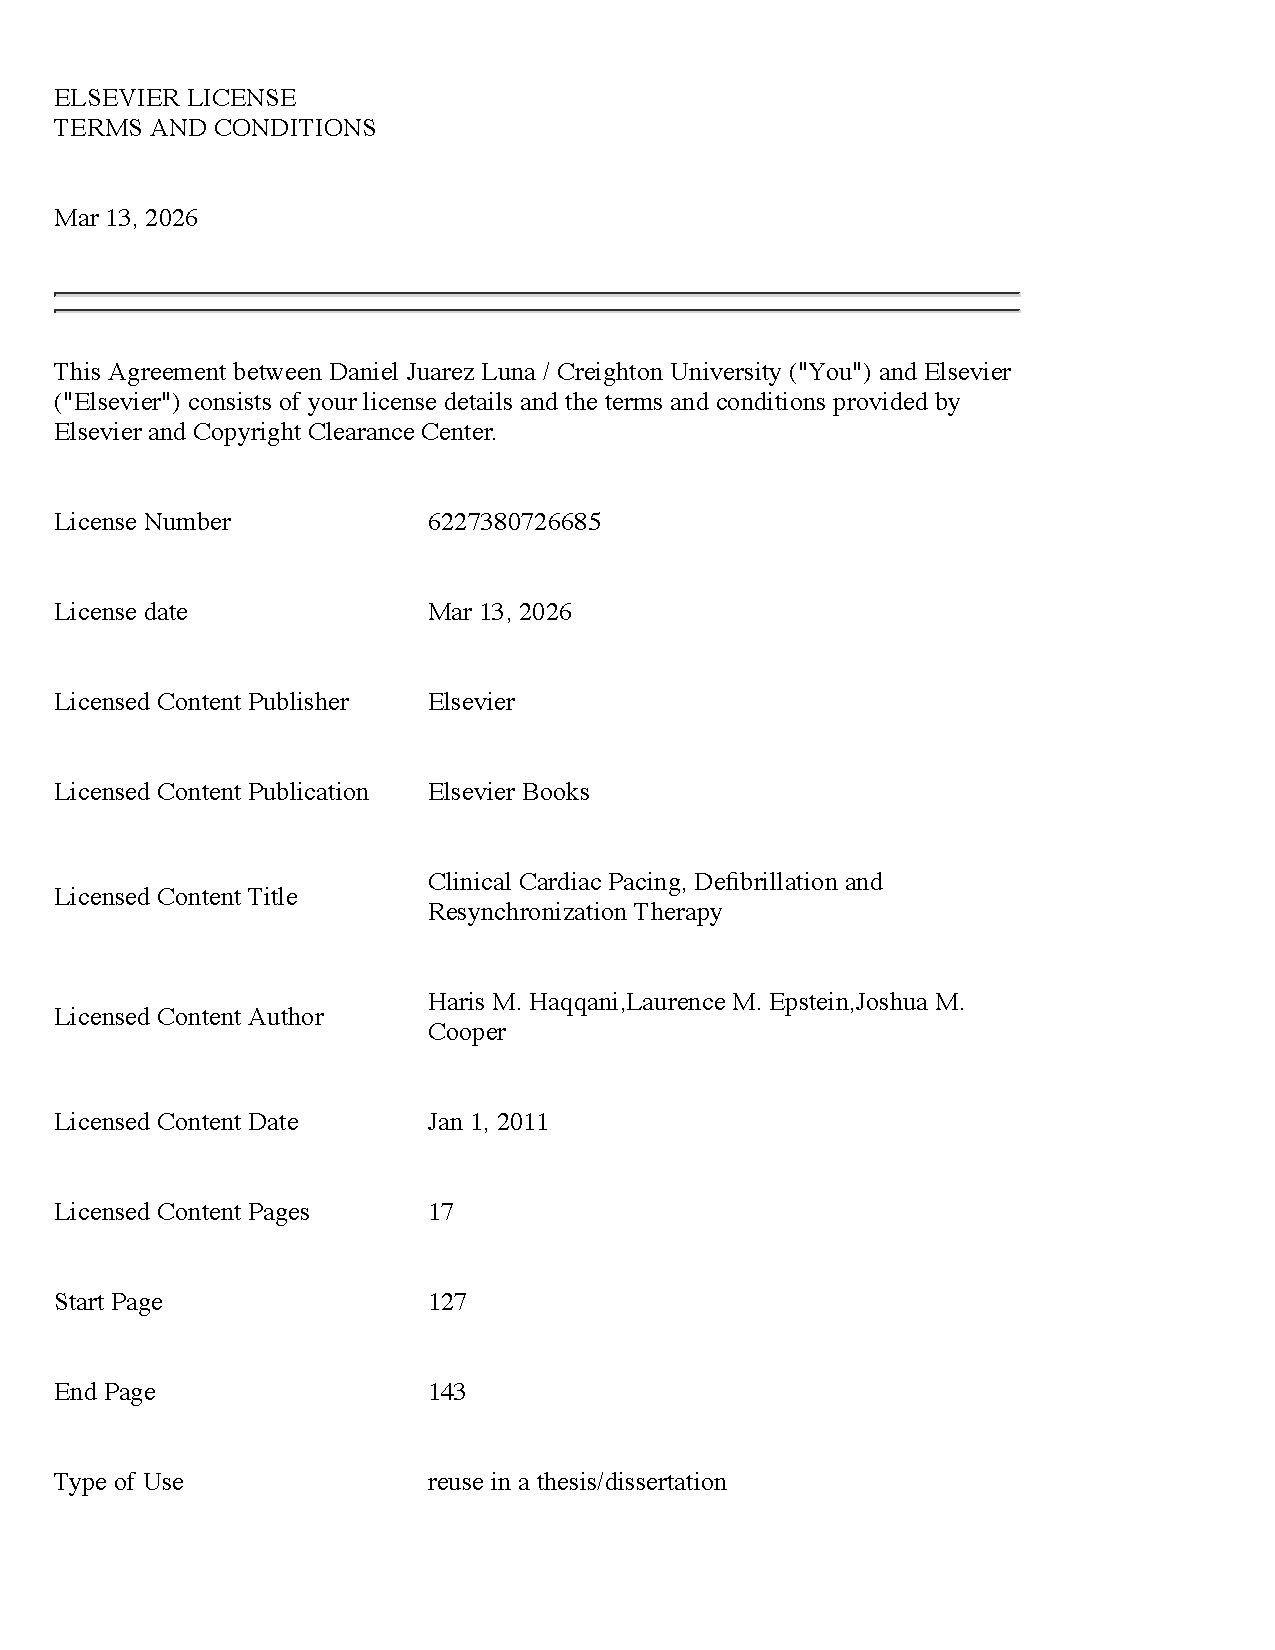
\includepdf[pages={1,2}, scale=0.90, offset=27mm 0mm]{Licenses/RightsLink Printable License-Epileadsfigures.pdf}


\invisiblesection{Appendix F2: Copyright License – Figure \ref{fig:astm_diagram}}
\label{app:B2}

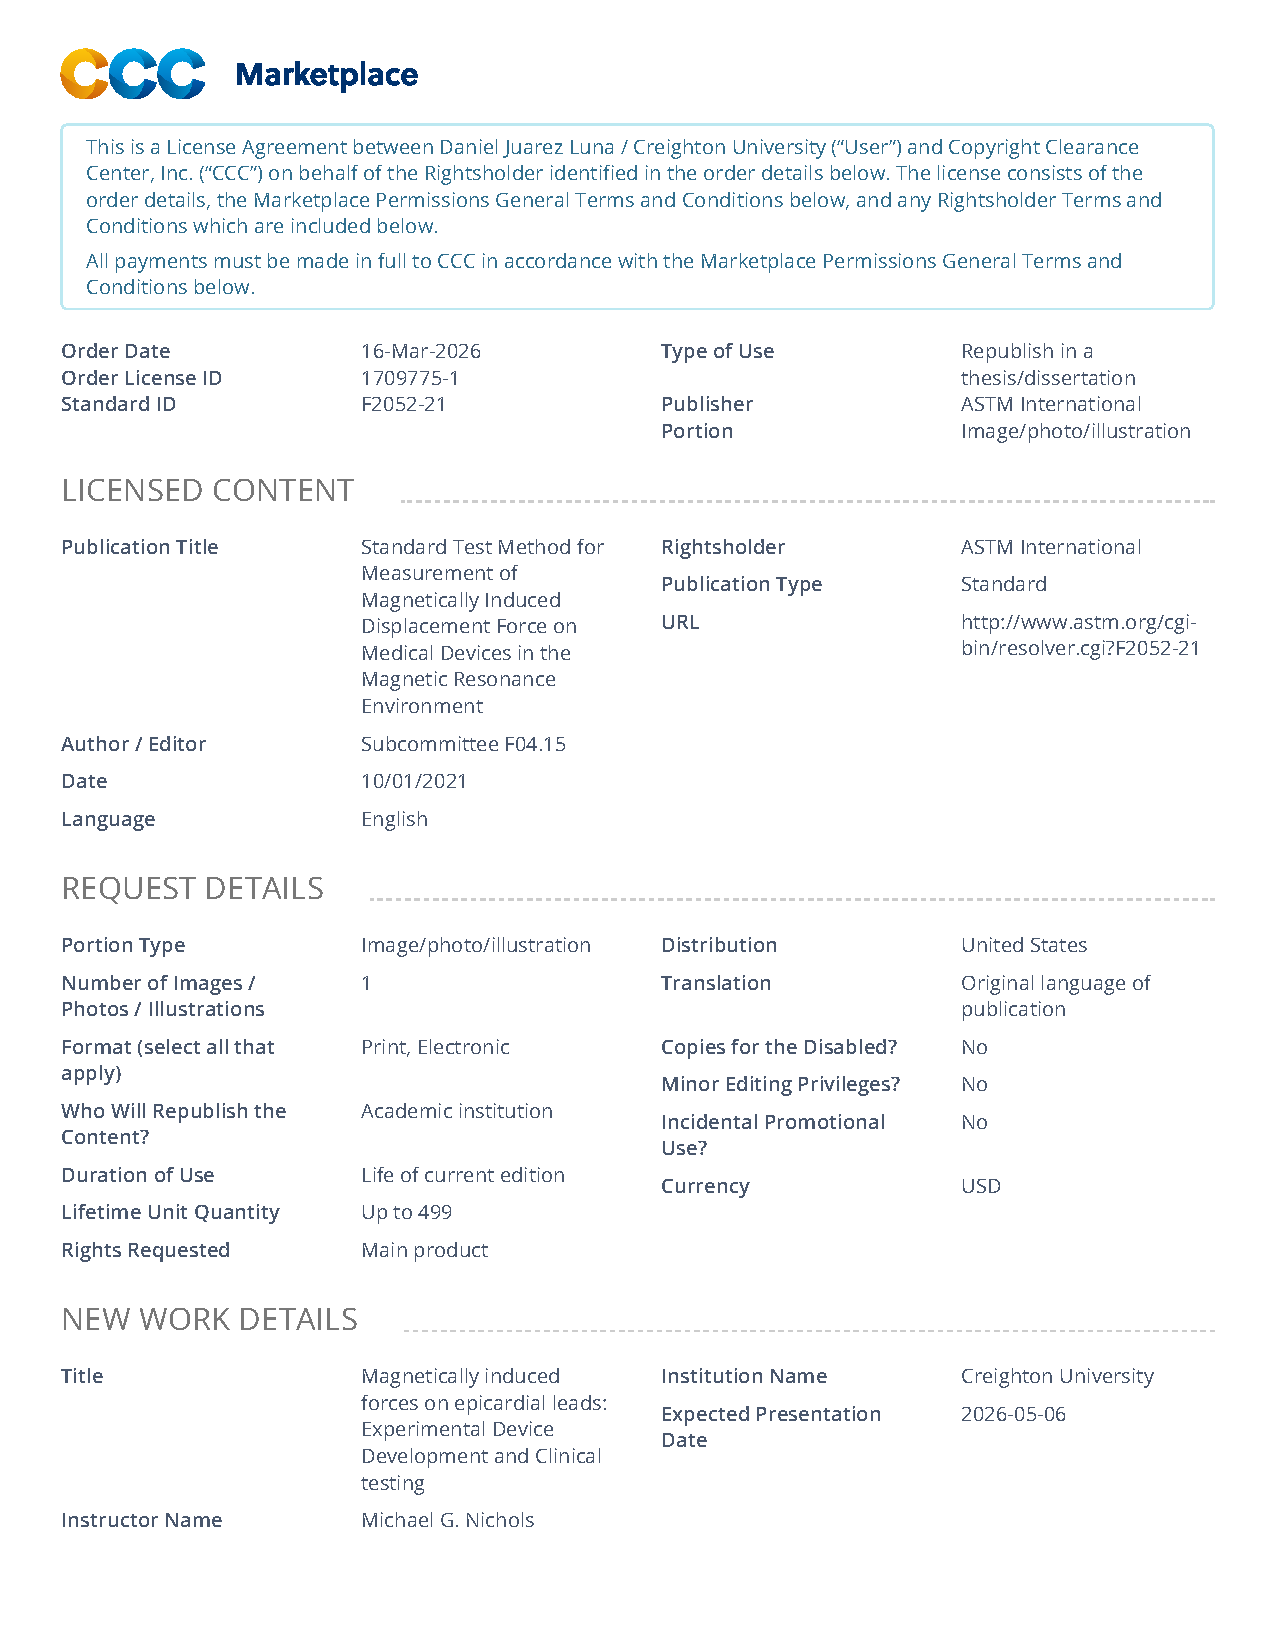
\includepdf[pages={1,2}, offset=13mm 0mm,  scale=0.90]{Licenses/ASTMF2052 License.pdf}